\section{Self-Reflection}

Even though the start of the implementation phase was a bit rocky, with time the author developed a deep understanding of all the tools and technologies required to build this project and manage to implement all the core functionalities to a high standard. One of the main goals the author has set up for themselves was to build this entire system be efficient as possible. Figure \ref{fig:service-benchmark} shows the resource usage of four services that a provisioned as part of this system while running under heavy load. Even then all four components combined don't use over 200MB of Memory and less than 0.1\% of the total CPUs available.

\begin{figure}[H]
    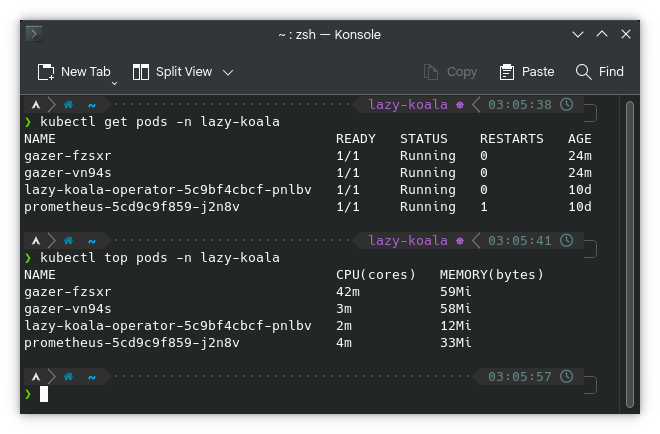
\includegraphics[width=15cm]{assets/implementation/service-benchmark.png}
    \caption{Resource usage of Lazy-Koala components (self-composed)}
    \label{fig:service-benchmark}
\end{figure}

At the current stage of the project, all the functionality of \ac{gazer} is implemented properly and telemetry scraping works as expected (Refer Appendix \ref{appendix:prometheus-dashboard} for Prometheus dashboard). Although some of the functionality of the \ac{lazy-koala-operator} was left out due to the limited time, notably the \ac{lazy-koala-operator} doesn't provision an instance of \ac{sherlock} due to the fact that model delivery process hasn't been finalized.

Initial results of \ac{sherlock} show that the author's hypothesis about the machine learning model architecture is feasible. Figure \ref{fig:normal-state} show encoded metric status while the system was stable and the reconstruction from \ac{sherlock} shows a similar output. This means reconstruction error is low hence the lower anomaly score. When it comes to \ref{fig:abnormal-state} there is a large difference between the input and output data frames. This is because the model hasn't seen metric levels like these and trying to stick to what it has been trained on. Hence the large reconstruction error.

\begin{figure}[H]
    \centering
    \begin{subfigure}[b]{0.7\textwidth}
        \centering
        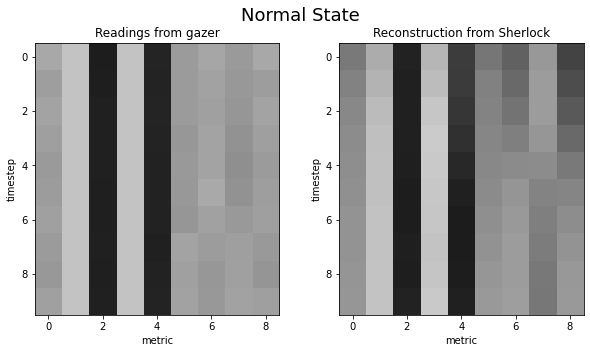
\includegraphics[width=\textwidth]{assets/implementation/normal-state.png}
        \caption{Normal State}
        \label{fig:normal-state}
    \end{subfigure}
    \hfill
    \begin{subfigure}[b]{0.7\textwidth}
        \centering
        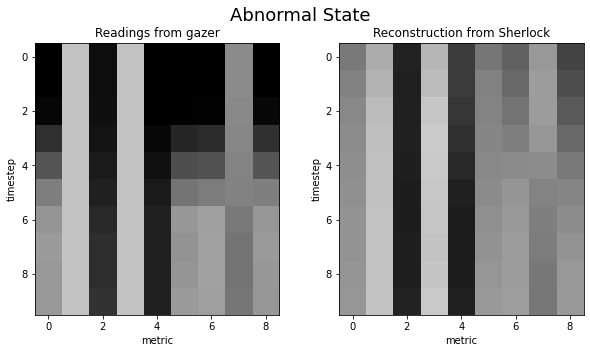
\includegraphics[width=\textwidth]{assets/implementation/abnormal-state.png}
        \caption{Abnormal State}
        \label{fig:abnormal-state}
    \end{subfigure}
    \hfill
       \caption{Initial results of the \ac{sherlock} model (self-composed)}
\end{figure}

\section{Video Demo}

The explanation of the research and video demonstration of the project can be found from here \href{https://www.youtube.com/watch?v=d5C2qLK1rG8}{https://www.youtube.com/watch?v=d5C2qLK1rG8}